\documentclass[../AnalysisNoteJBuxton.tex]{subfiles}
\begin{document}

\subsection{Pair Selection}
\label{PairSelection}

It is important to obtain true particle pairs in the analysis.  In particular, contamination from pairs constructed with split or merged tracks, and pairs sharing daughters, can introduce an artificial signal into the correlation function, obscuring the actual physics.

\begin{enumerate}
 \item Shared Daughter Cut for Pairs
 \begin{enumerate}
  \item V0-V0 Pairs (i.e. $\Lambda$($\bar{\Lambda}$)K$^{0}_{S}$ analyses)
  \begin{itemize}
   \item Remove all pairs which share a daughter 
   \begin{itemize}
    \item Ex. $\Lambda$ and K$^{0}_{S}$ particles which share a $\pi^{-}$ daughter are not included
   \end{itemize} 
  \end{itemize}
  \item V0-Track Pairs (i.e. $\Lambda$($\bar{\Lambda}$)K$^{\pm}$ analyses)
  \begin{itemize}
   \item Remove pairs if Track is also used as a daughter of the V0
   \begin{itemize}
    \item In these analyses, this could only occur if, for instance, a $K$ is misidentified as a $\pi$ or $p$ in the V0 reconstruction
   \end{itemize}
  \end{itemize}
  \item $\Xi$-Track Pairs
  \begin{itemize}
   \item Remove pairs if Track is also used as a daughter of the $\Xi$
   \begin{itemize}
    \item In these analyses, this could only occur if, for instance, a $K$ is misidentified as a $\pi$ or $p$ in the V0 reconstruction, or misidentified as bachelor $\pi$.
   \end{itemize}
   \item Remove pair if bachelor $\pi$ is also a daughter of the $\Lambda$
   \begin{itemize}
    \item This is not a pair cut, but is included here because this cut occurs in the \\AliFemtoXiTrackPairCut class
   \end{itemize}
  \end{itemize}  
 \end{enumerate}
 \item Average Separation Cuts
 \begin{itemize}
  \item Used to cut out splitting and merging effects
  \item The motivation for these cuts can be seen in Figures \ref{fig:AvgSepLamK0}, \ref{fig:AvgSepLamKch}, and \ref{fig:AvgSepXiKch}, in which average separation correlation functions are presented
 \end{itemize}
 \begin{enumerate}
  \item $\Lambda$($\bar{\Lambda}$)K$^{0}_{S}$ Analyses
  \begin{itemize}
   \item Average separation $>$ 6.0 cm for like charge sign daughters
   \begin{itemize}
    \item ex. $p$ daughter of $\Lambda$ and $\pi^{+}$ daughter of K$^{0}_{S}$
   \end{itemize}
   \item No cut for unlike-sign daughters
  \end{itemize}
  \item $\Lambda$($\bar{\Lambda}$)K$^{\pm}$ Analyses
  \begin{itemize}
   \item Average Separation $>$ 8.0 cm for daughter of $\Lambda$($\bar{\Lambda}$) sharing charge sign of K$^{\pm}$
   \begin{itemize}
    \item ex. in $\Lambda$K$^{+}$ analysis, $p$ daughter of $\Lambda$ with K$^{+}$
   \end{itemize}
   \item No cut for unlike signs
  \end{itemize}
  \item $\Xi$($\bar{\Xi}$)K$^{\pm}$ Analyses
  \begin{itemize}
   \item Average Separation $>$ 8.0 cm for any daughter of $\Xi$ sharing charge sign of K$^{\pm}$
   \begin{itemize}
    \item ex. in $\Xi^{-}$K$^{-}$ analysis, $\pi^{-}$ daughter of $\Lambda$ daughter with K$^{-}$, and bachelor $\pi^{-}$ daughter with K$^{-}$
   \end{itemize}
   \item No cut for unlike signs
  \end{itemize}  
 \end{enumerate}
\end{enumerate}

\begin{figure}[h]
  \centering
  \includegraphics[width=0.8\textwidth]{3_DataSelection/Figures/AvgSepCFs_LamK0.pdf}
  \caption[Avgerage Separation of $\Lambda$($\bar{\Lambda}$) and K$^{0}_{S}$ Daughters]{Avgerage separation (cm) correlation functions of $\Lambda$($\bar{\Lambda}$) and K$^{0}_{S}$ Daughters.  Only like-sign daughter pairs are shown (the distributions for unlike-signs were found to be flat).  The title of each subfigure shows the daughter pair, as well as the mother of each daughter (in ``()"),  ex. top left is p from $\Lambda$ with $\pi^{+}$ from K$^{0}_{S}$.}
  \label{fig:AvgSepLamK0}
\end{figure}

\begin{figure}[h]
  \centering
  \includegraphics[width=0.8\textwidth]{3_DataSelection/Figures/AvgSepCFs_LamKch.pdf}
  \caption[Avgerage Separation of $\Lambda$($\bar{\Lambda}$) Daughter and K$^{\pm}$]{Avgerage separation (cm) correlation functions of $\Lambda$($\bar{\Lambda}$) Daughter and K$^{\pm}$.  Only like-sign pairs are shown (unlike-signs were flat).  In the subfigure titles, the particles in ``()" represent the mothers, ex. top left is p from $\Lambda$ with K$^{+}$.}
  \label{fig:AvgSepLamKch}
\end{figure}



\begin{figure}[h]
  \centering
  %%----start of first subfigure---  
  \subfloat[$\Xi^{-}$K$^{+}$]{
    \label{fig:AvgSepXiKch:a}
    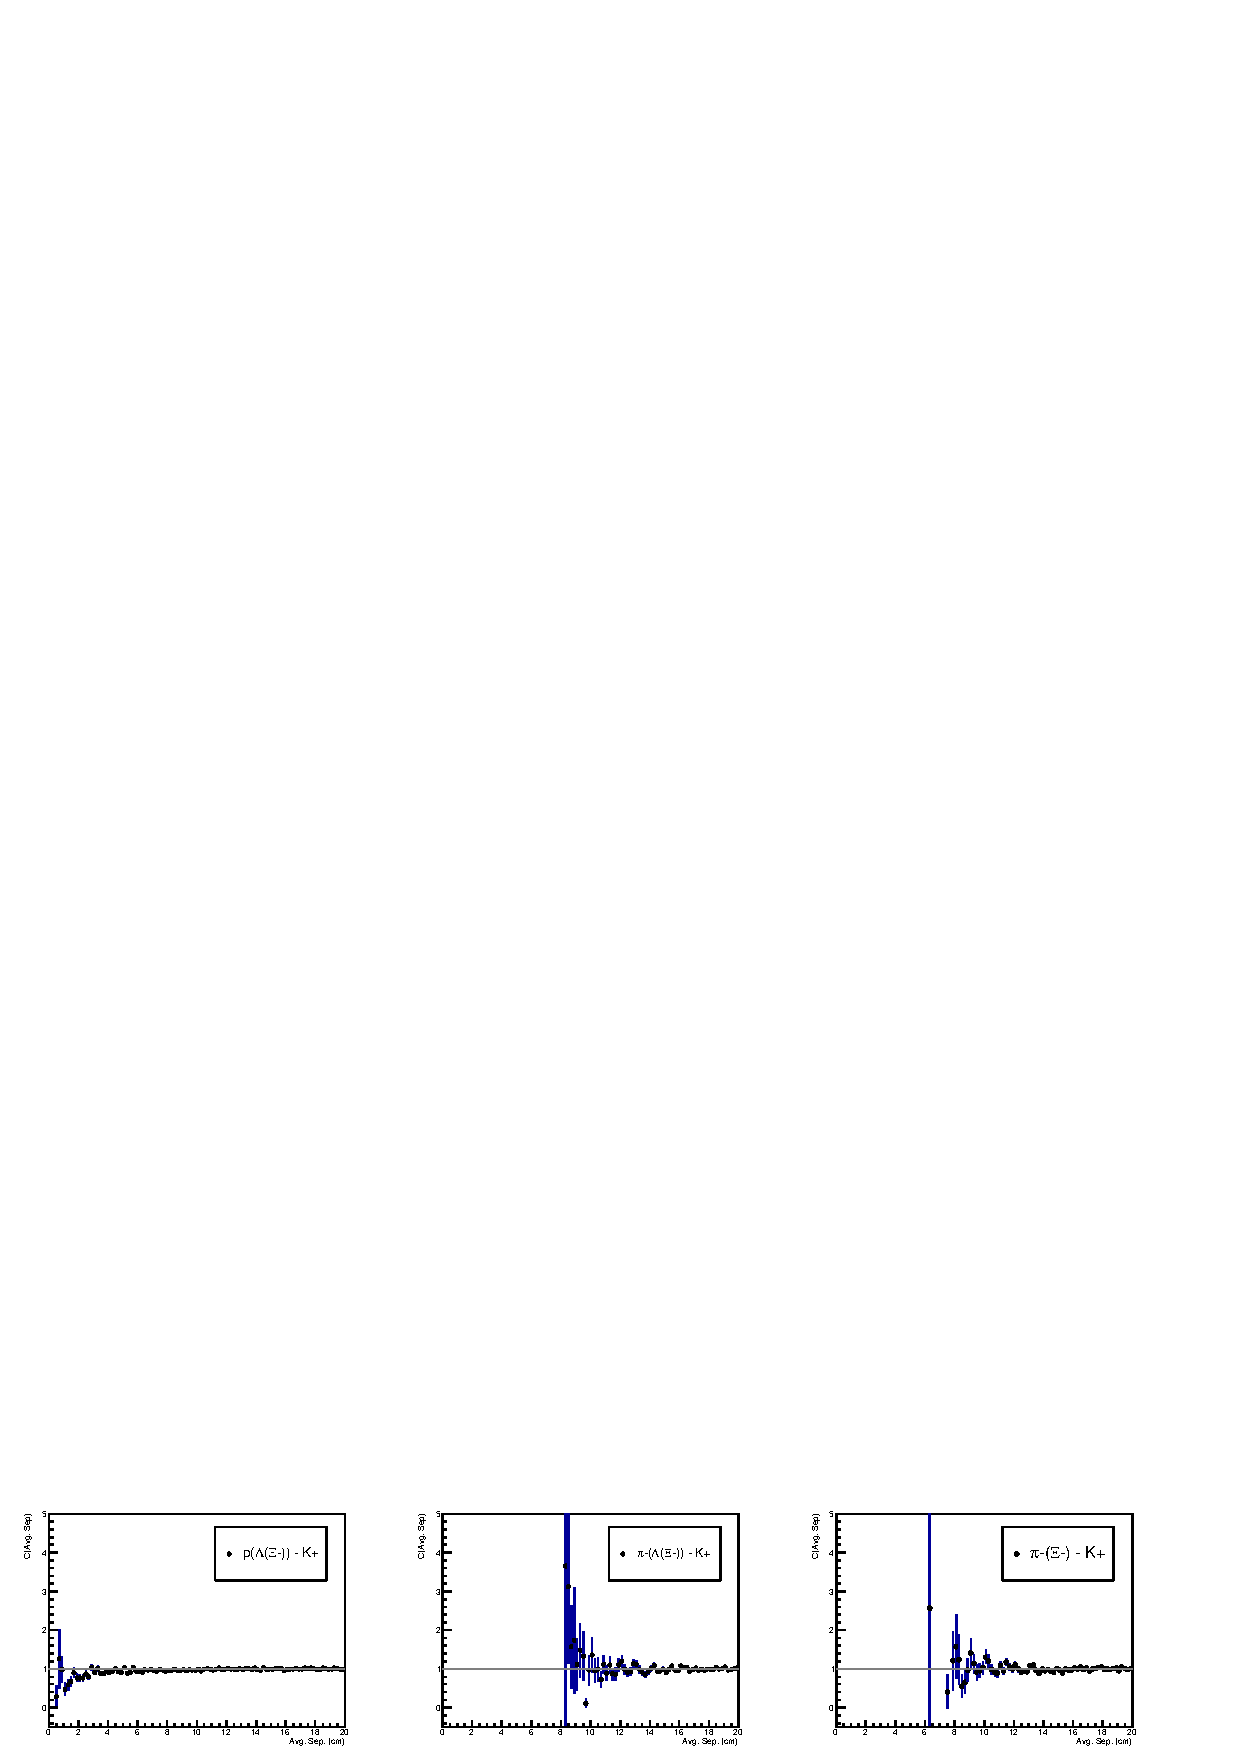
\includegraphics[width=0.99\textwidth]{3_DataSelection/Figures/cXicKchAvgSepCfs_XiKchP.pdf}}\\
  %%----start of second subfigure---
  \subfloat[$\bar{\Xi}^{+}$K$^{-}$]{
    \label{fig:AvgSepXiKch:b}
    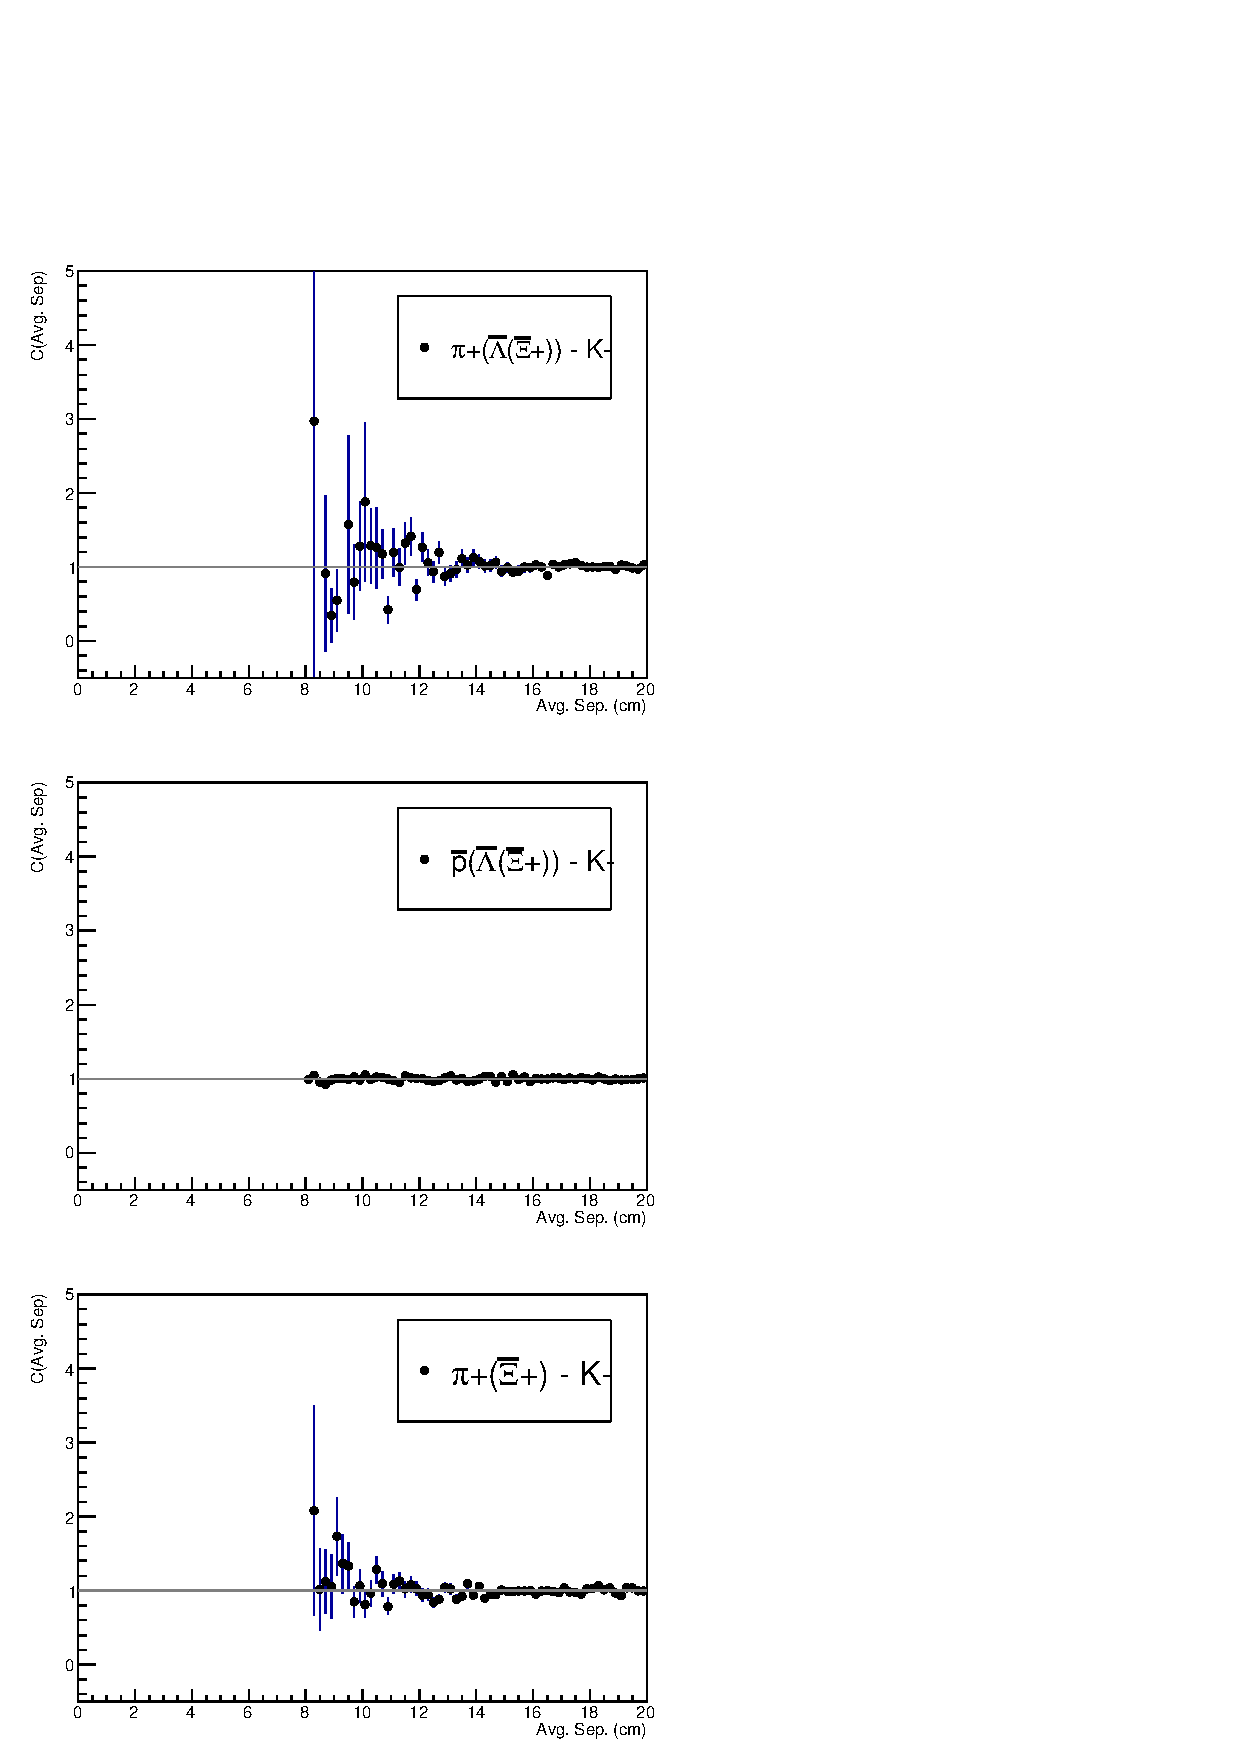
\includegraphics[width=0.99\textwidth]{3_DataSelection/Figures/cXicKchAvgSepCfs_AXiKchM.pdf}}\\
      %%----start of third subfigure---  
  \subfloat[$\Xi^{-}$K$^{-}$]{
    \label{fig:AvgSepXiKch:c}
    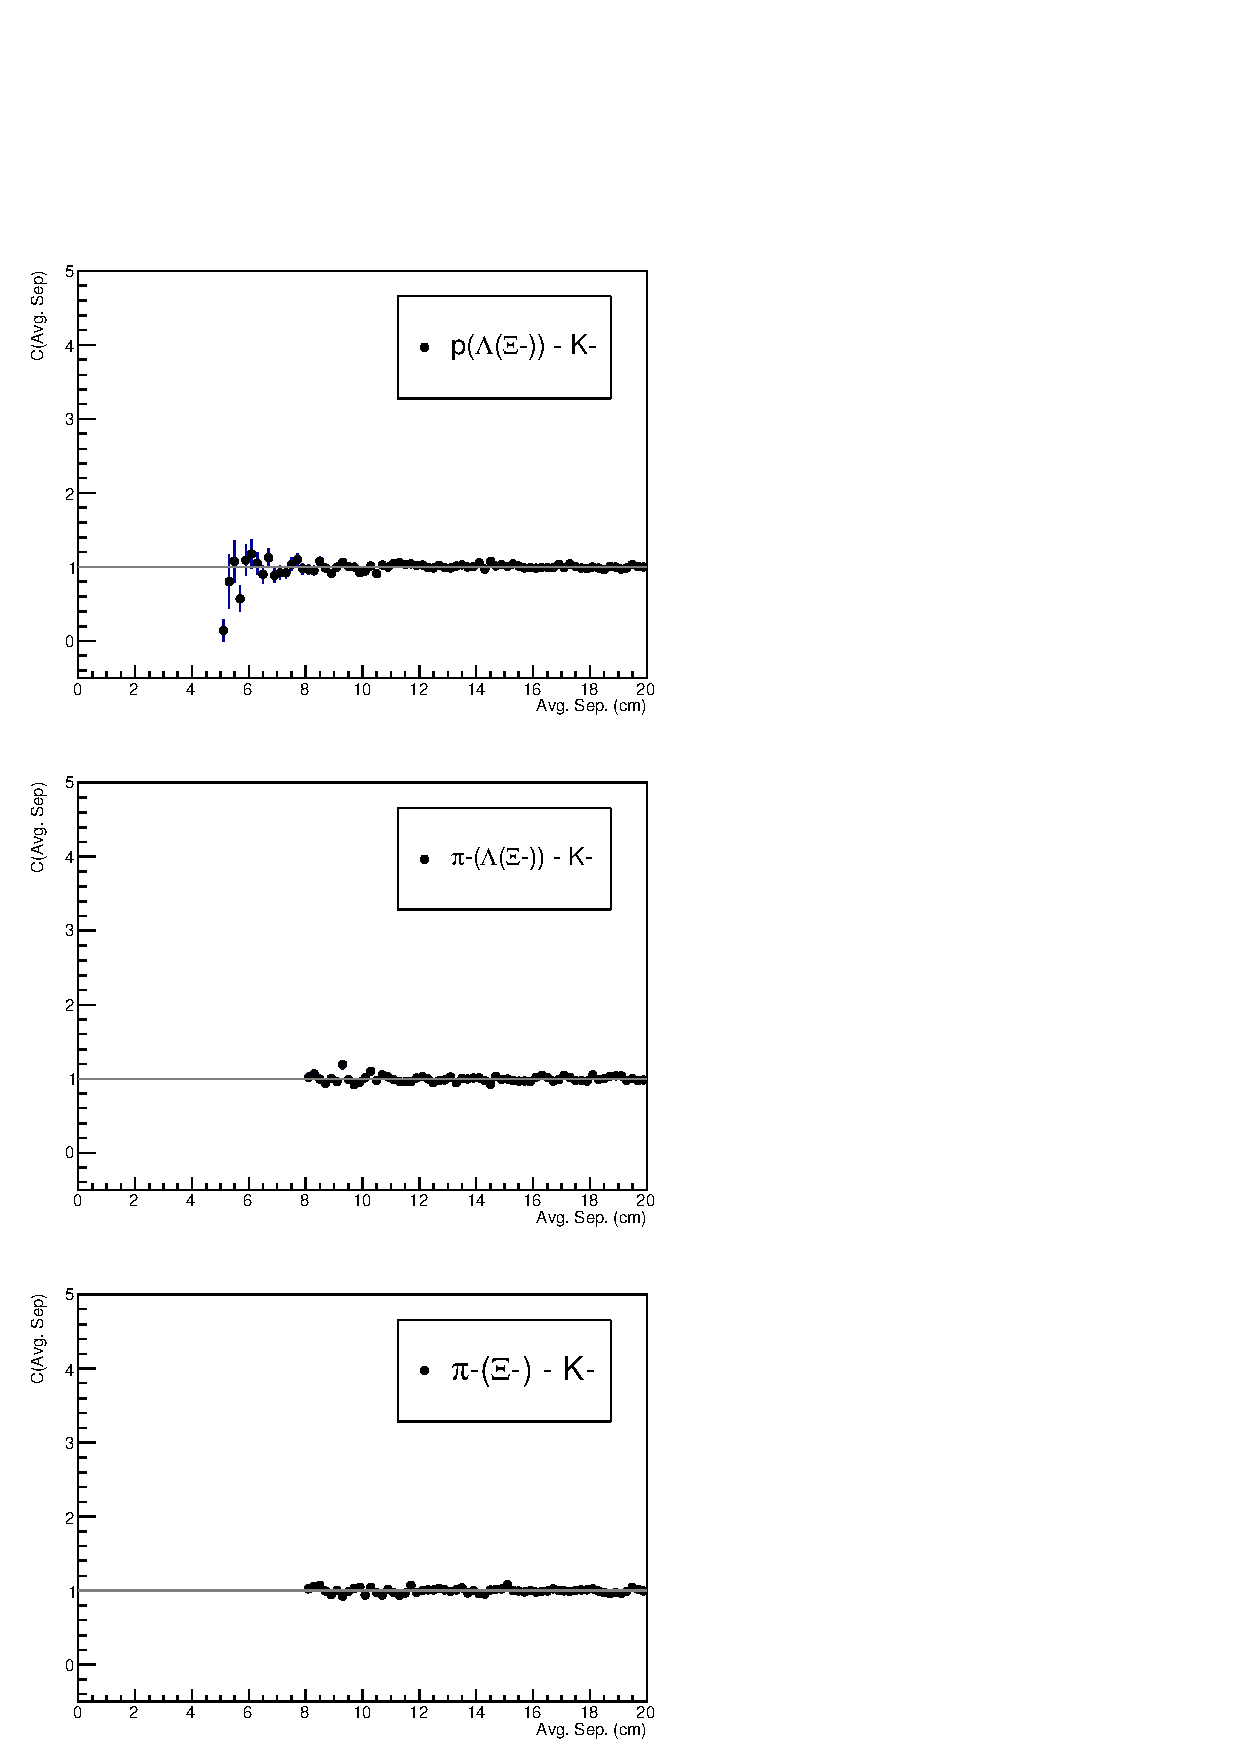
\includegraphics[width=0.99\textwidth]{3_DataSelection/Figures/cXicKchAvgSepCfs_XiKchM.pdf}}\\
  %%----start of fourth subfigure---
  \subfloat[$\bar{\Xi}^{+}$K$^{+}$]{
    \label{fig:AvgSepXiKch:d}
    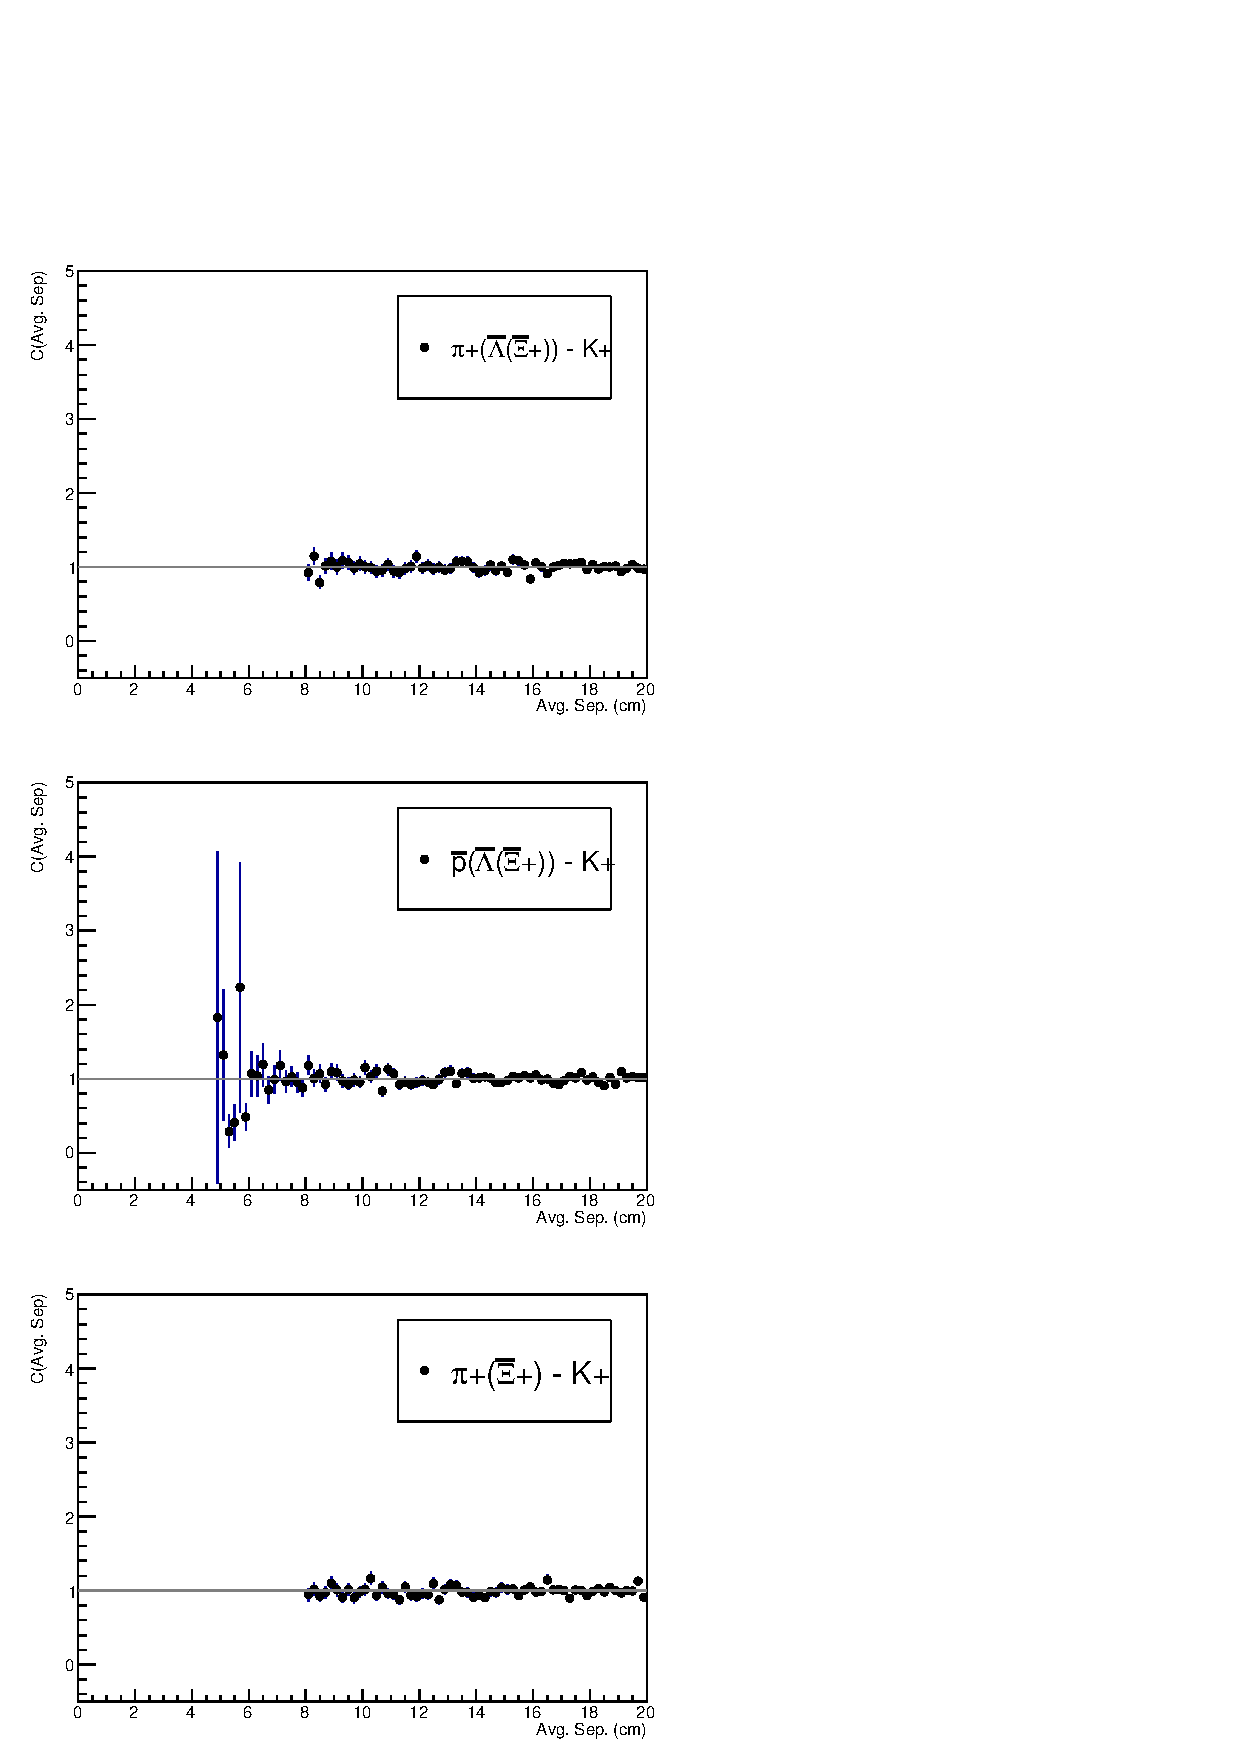
\includegraphics[width=0.99\textwidth]{3_DataSelection/Figures/cXicKchAvgSepCfs_AXiKchP.pdf}}
  %%----overall caption----
  \caption[Avgerage Separation of $\Xi$ Daughters and K$^{\pm}$]{Avgerage separation (cm) correlation functions of $\Xi$ Daughter and K$^{\pm}$.  In the subfigure titles, the particles in ``()" represent the mothers, ex. top left is p from $\Lambda$ from $\Xi^{-}$ with K$^{+}$.}
  \label{fig:AvgSepXiKch}
\end{figure}


\end{document}